Here we define the tools used to monitor and to check/validate alignment results. We also 
define the plots and the technical issues related to validation for later reference throughout 
the note.  
 
The approximate length is one page and about 4 figures. 

Test 1, figure ~\ref{fig:valid_DTconsts} shows blablabla.
\begin{figure}[h!]
  \centering
  \subfigure[]{
    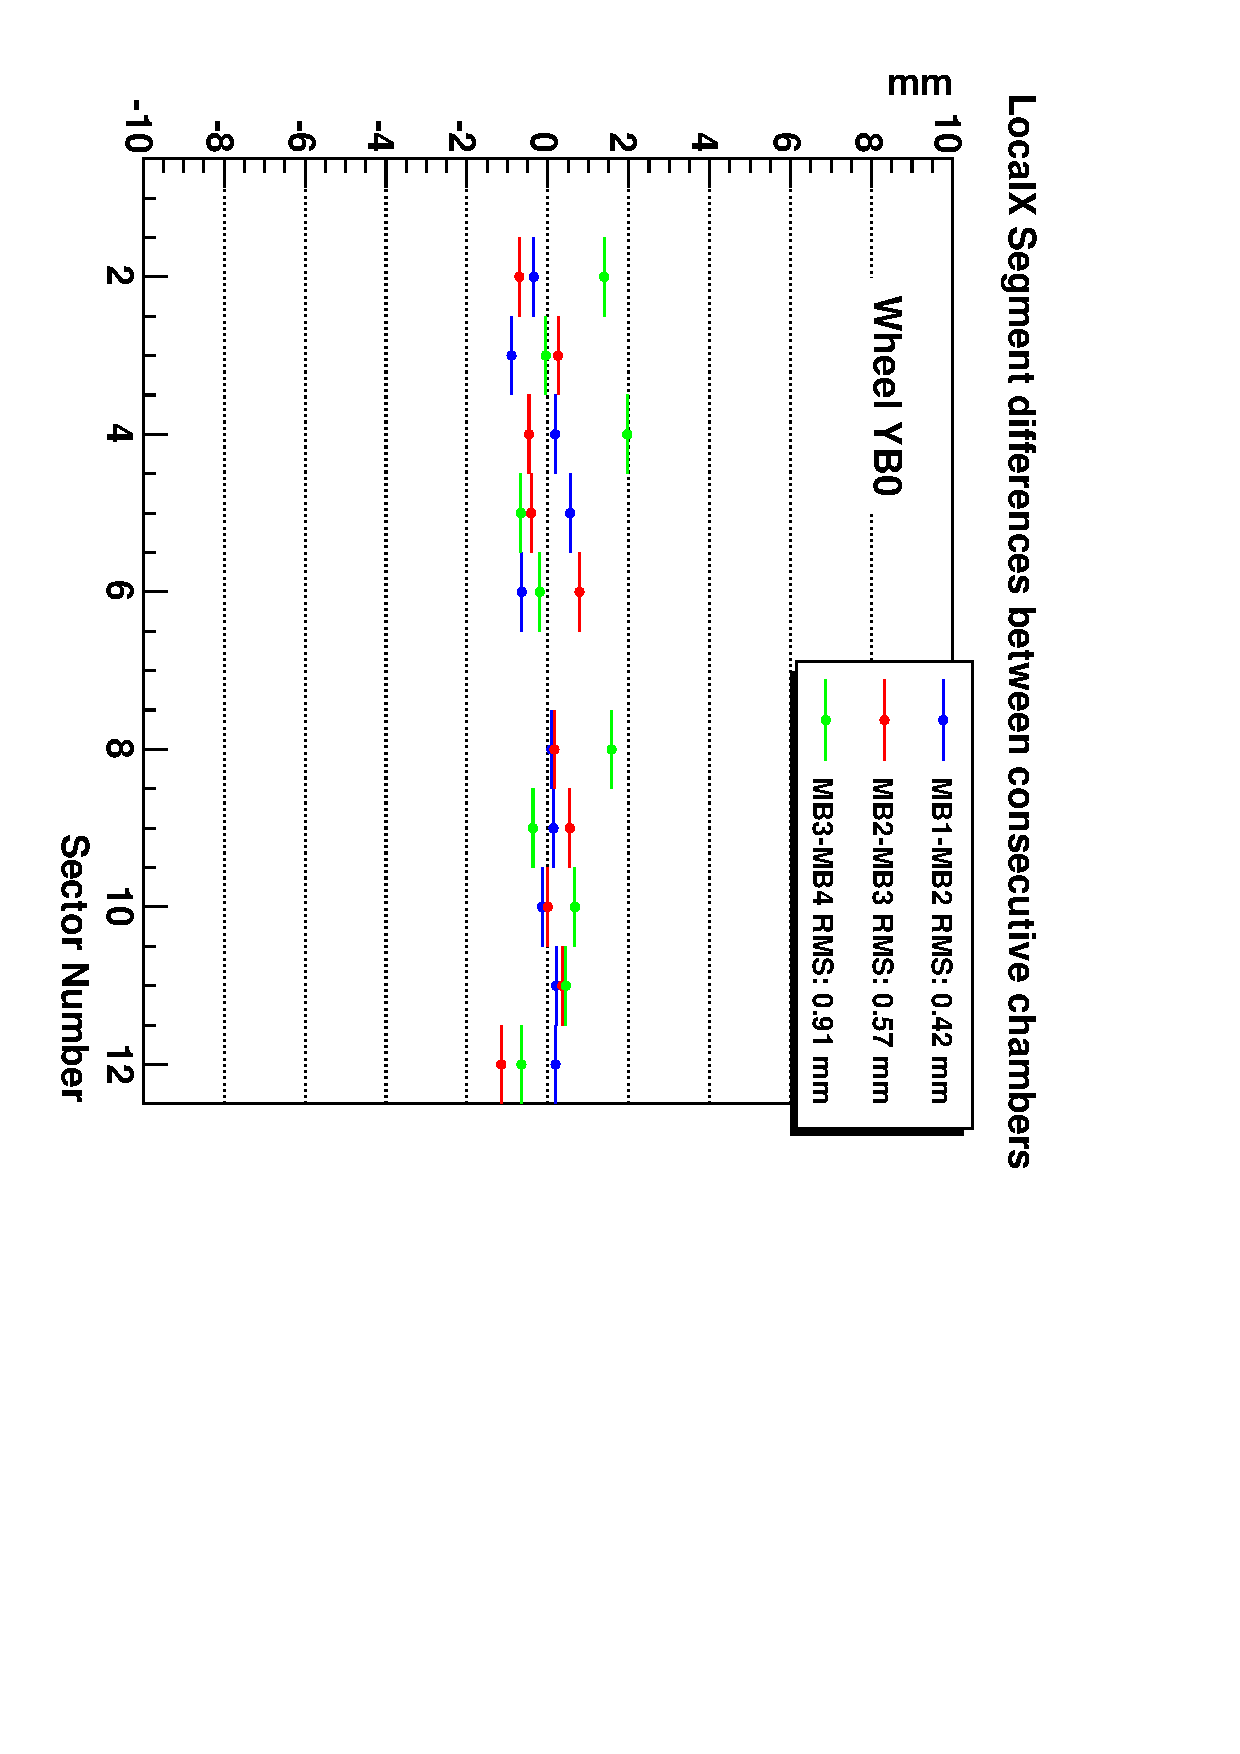
\includegraphics[width=0.4\textwidth, angle=90]{plots/validation/aligVal_08June09_LocalX_YB0.pdf}
  }
  \subfigure[]{
    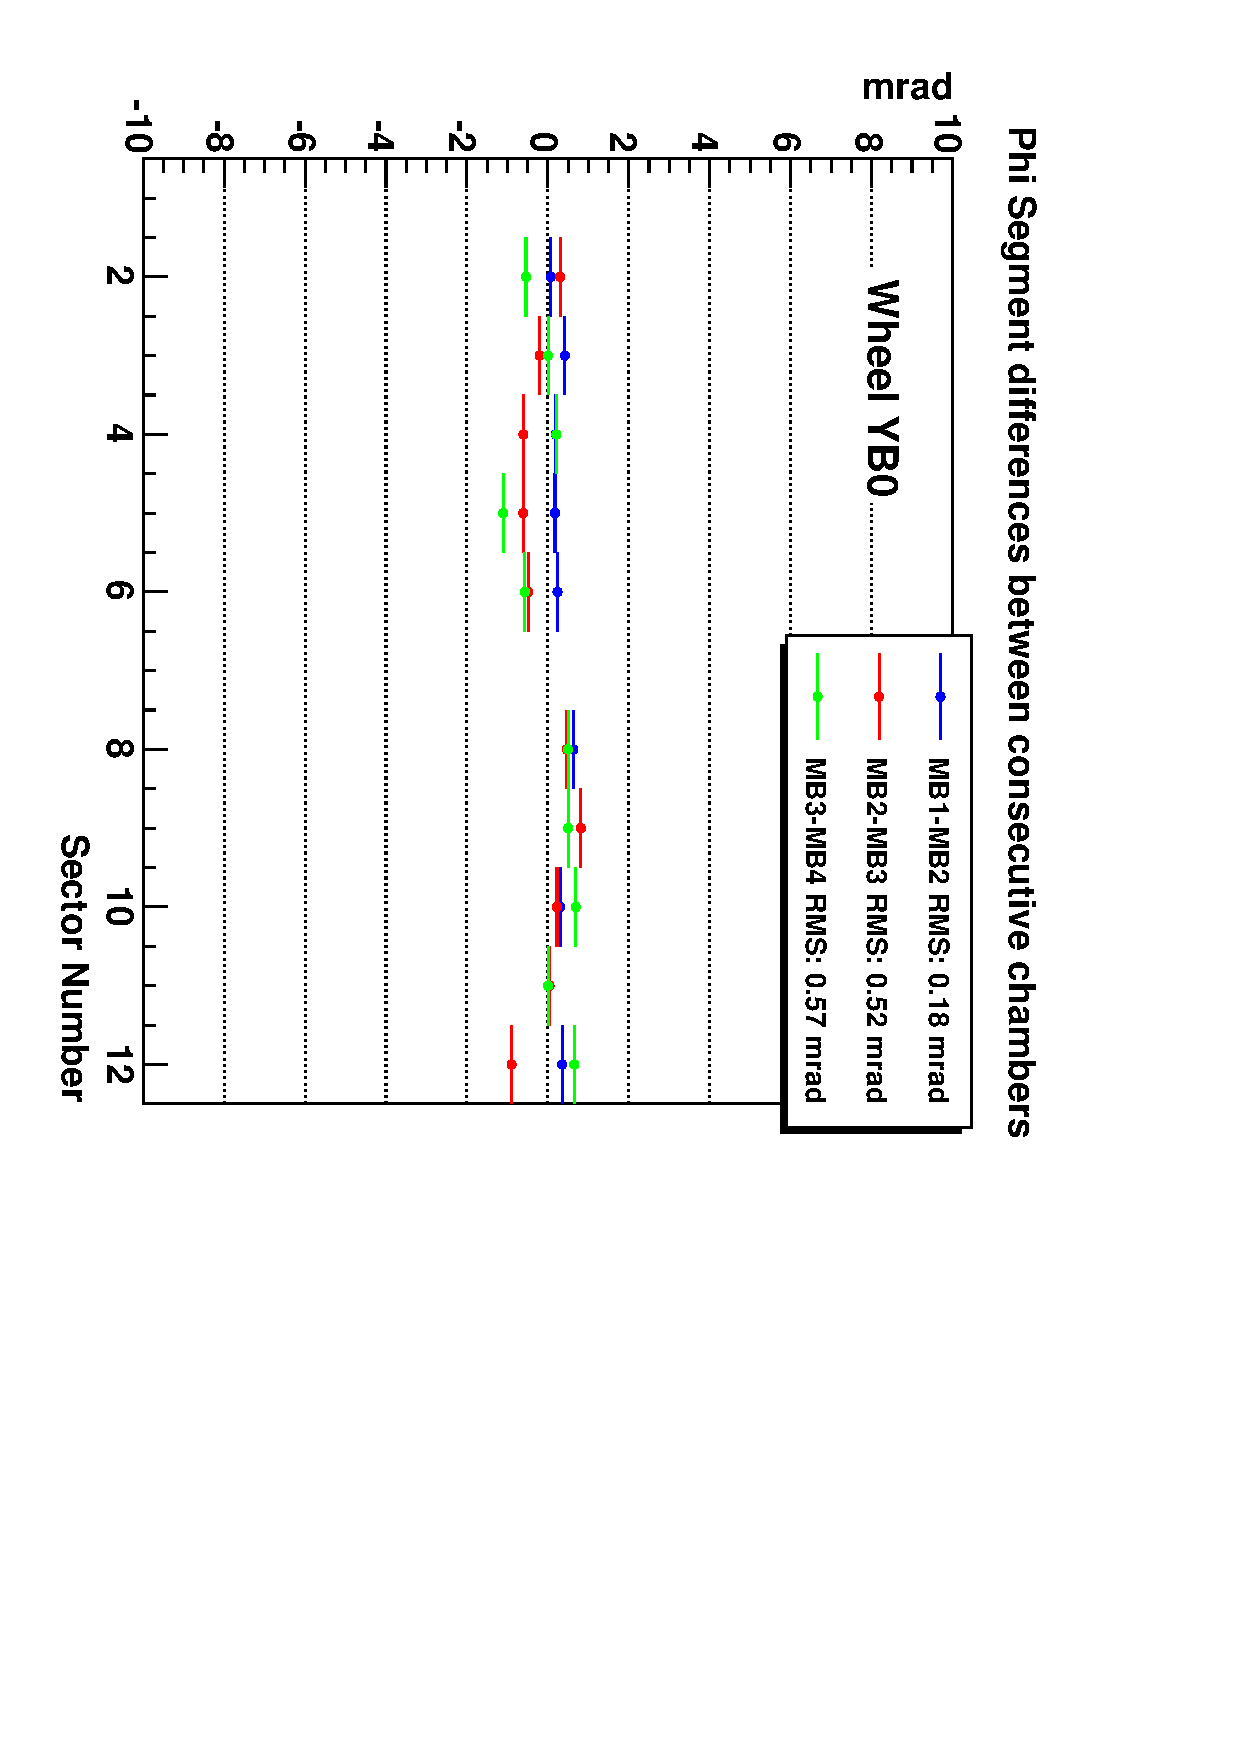
\includegraphics[width=0.4\textwidth, angle=90]{plots/validation/aligVal_08June09_Phi_YB0.pdf}
  }
  \label{fig:valid_DTconsts}
  \caption{The localx and phi validation from STA segment extrapolation }
\end{figure}
 
Test 2, figure ~\ref{fig:valid_NOMvsMPvsHIP} shows blablabla.
\begin{figure}[h!]
  \centering
  \subfigure[]{
    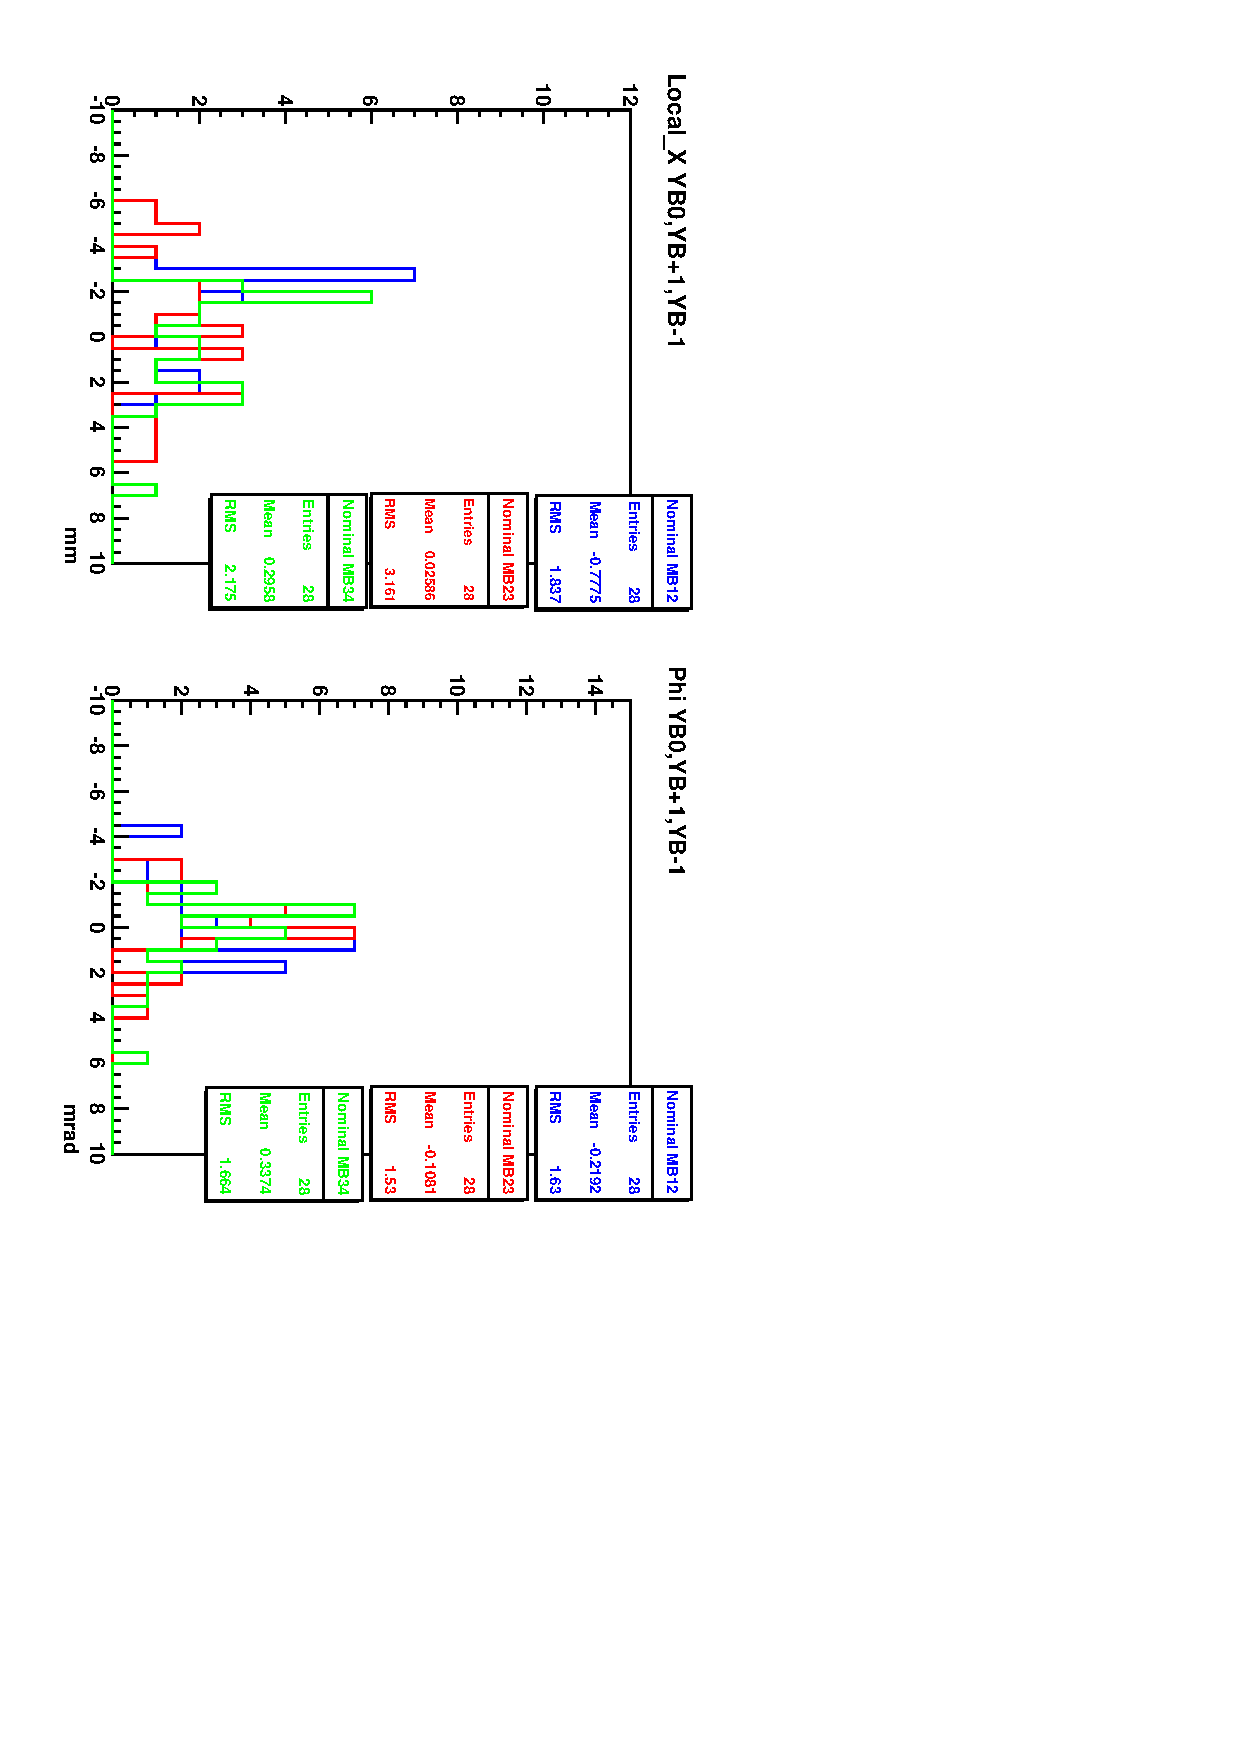
\includegraphics[width=0.4\textwidth, angle=90]{plots/validation/meanHisto_Nominal.pdf}
  }
  \subfigure[]{
    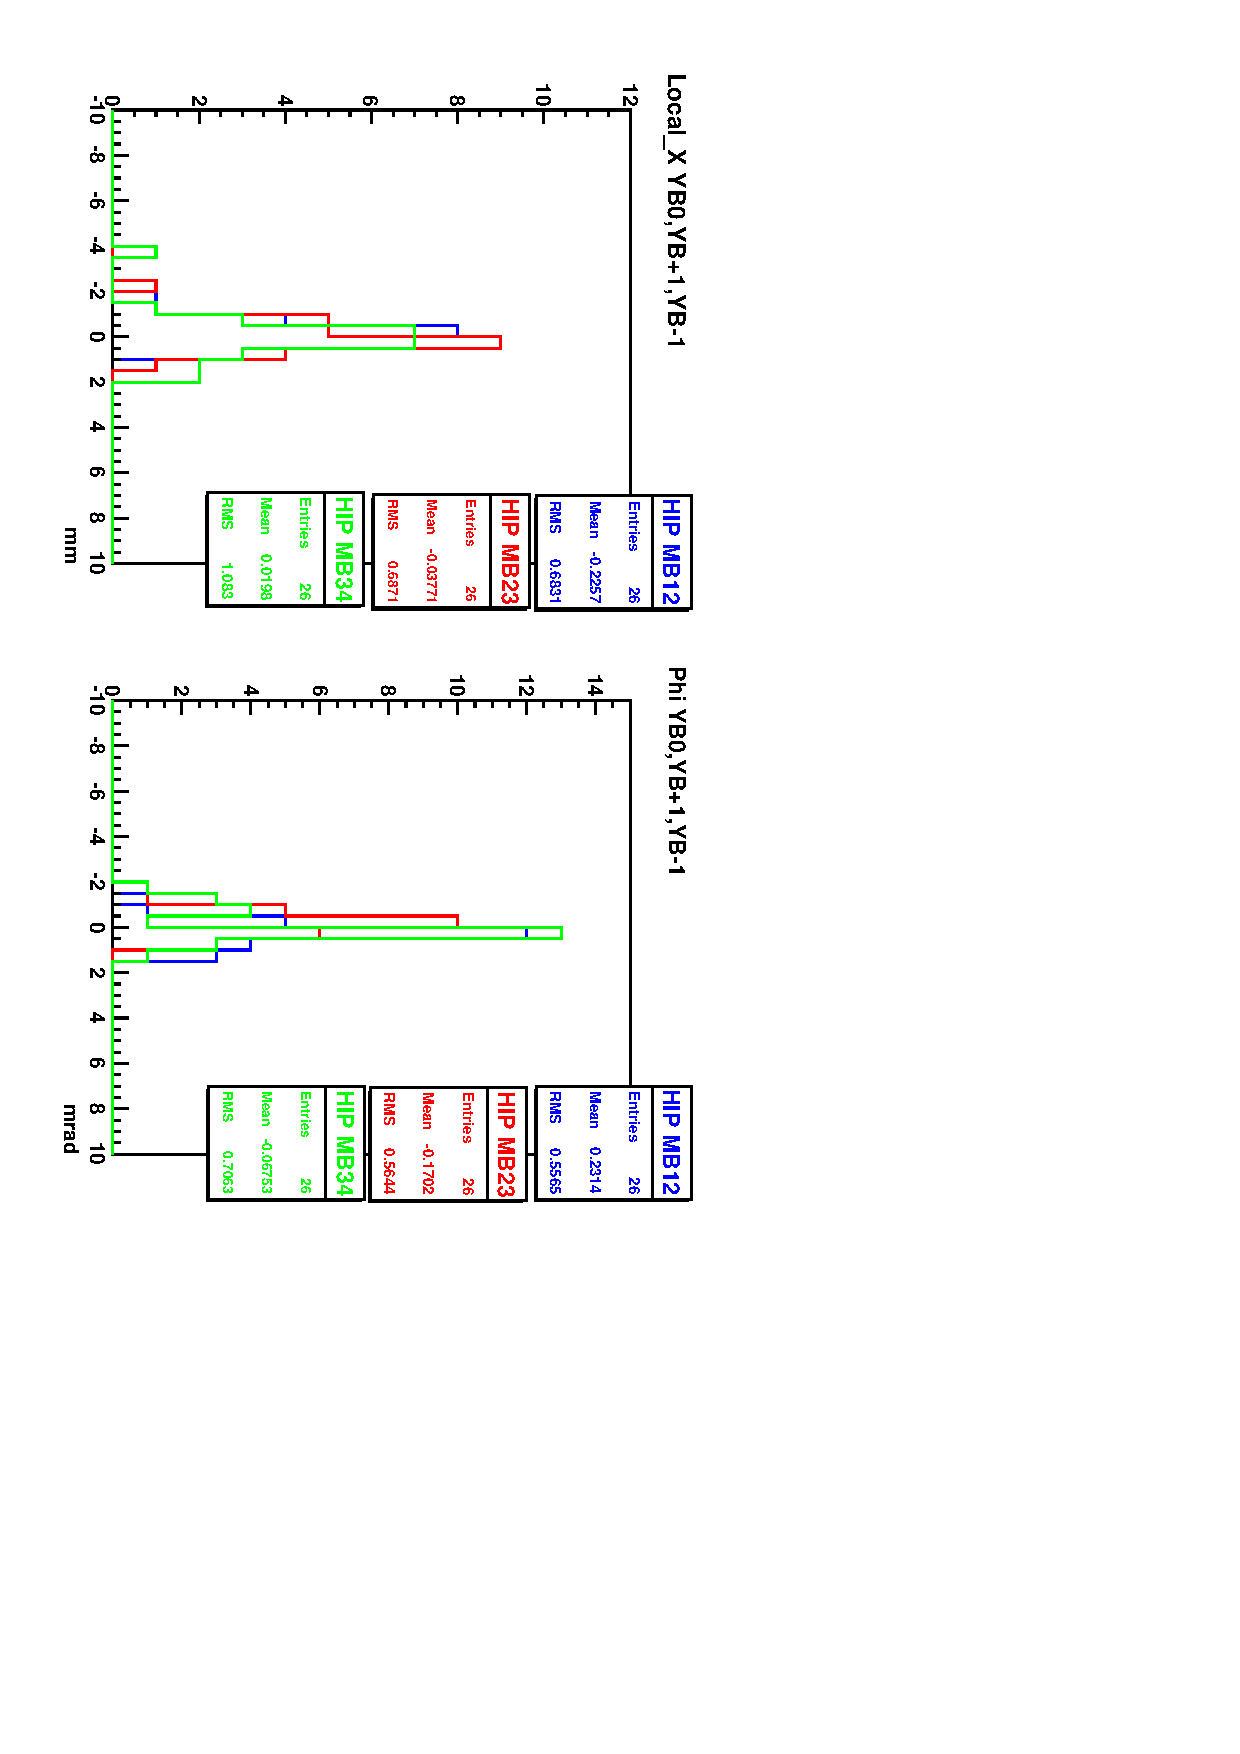
\includegraphics[width=0.4\textwidth, angle=90]{plots/validation/meanHisto_HIP_onlyAlign.pdf}
  }
  \subfigure[]{
    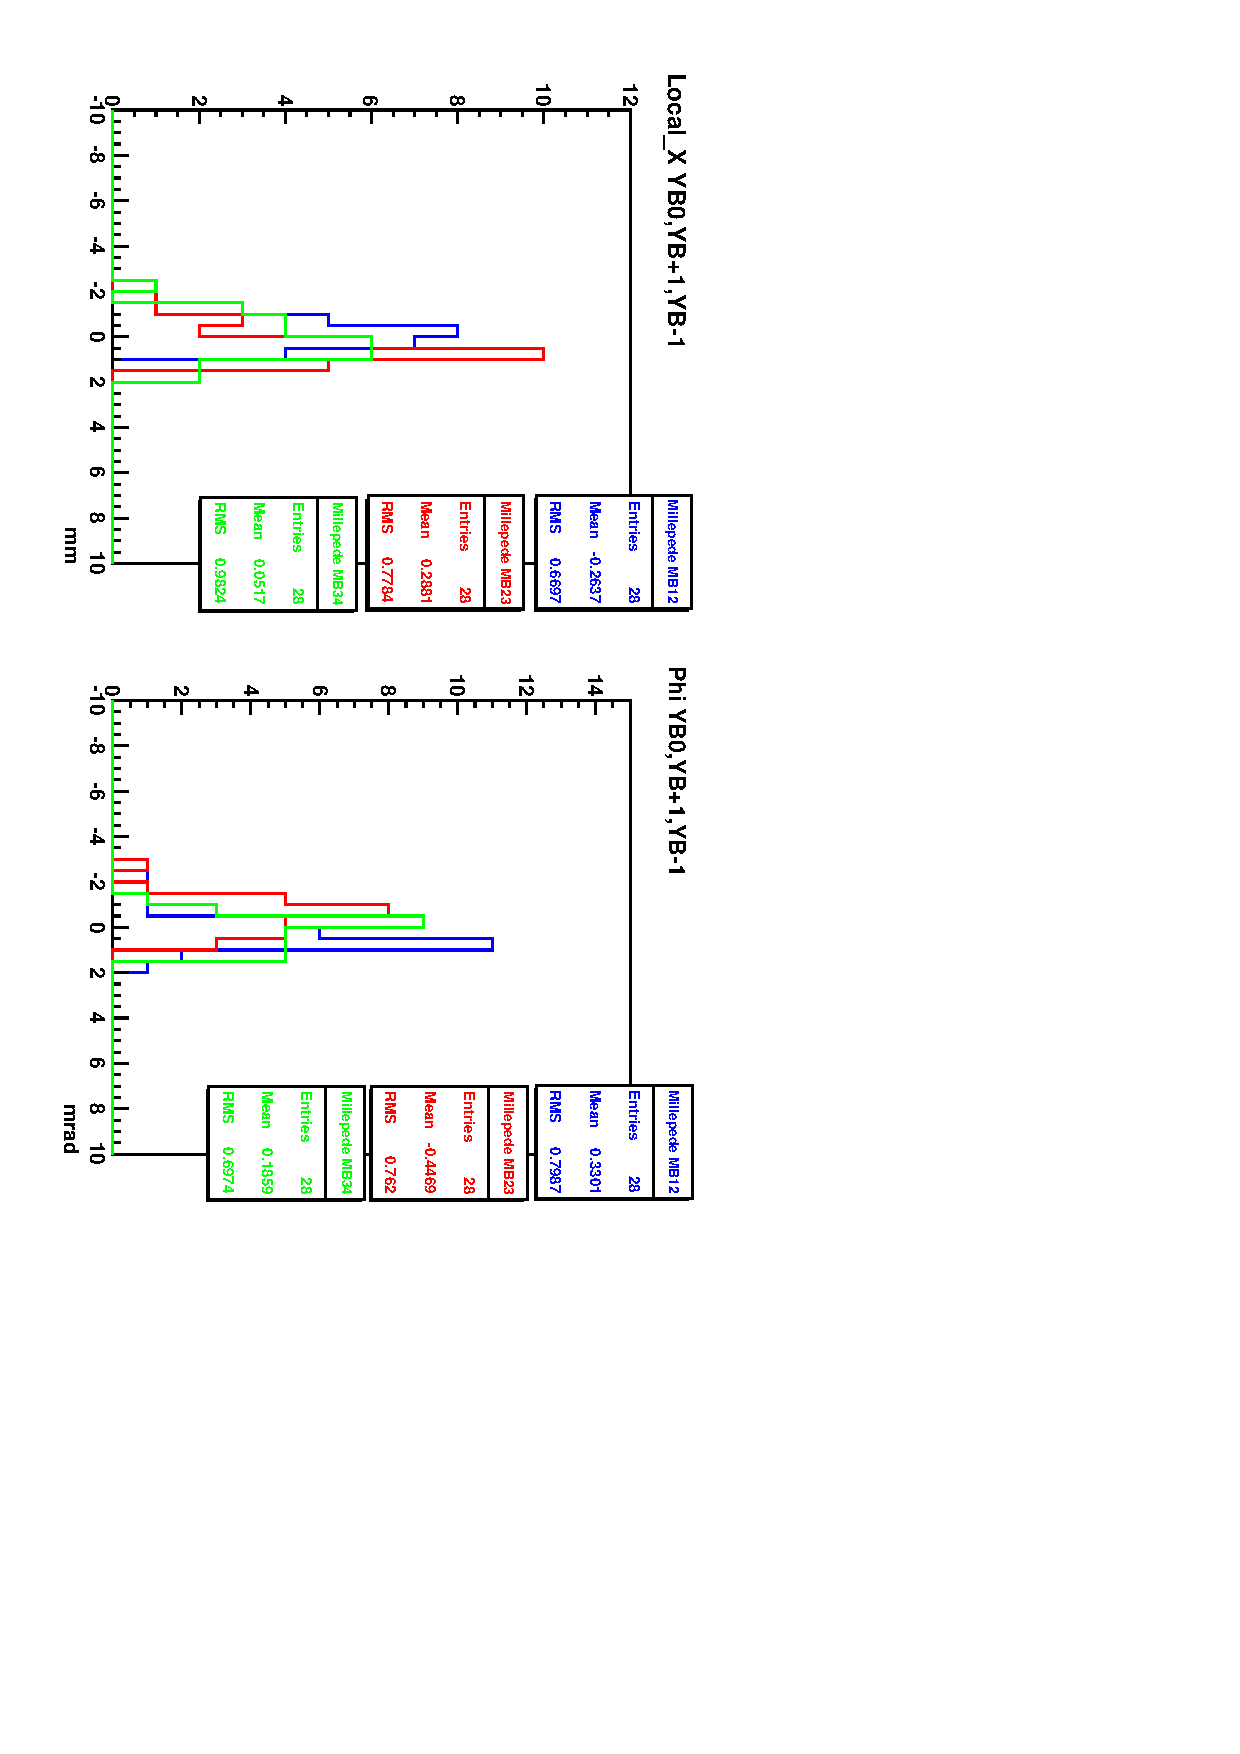
\includegraphics[width=0.4\textwidth, angle=90]{plots/validation/meanHisto_Millepede.pdf}
  }
  \label{fig:valid_NOMvsMPvsHIP}
  \caption{The localx and phi validation from STA segment extrapolation. }
\end{figure}
 
Test 3, figure ~\ref{fig:valid_RMDYB0} shows blablabla.
\begin{figure}[h!]
  \centering
  \subfigure[]{
    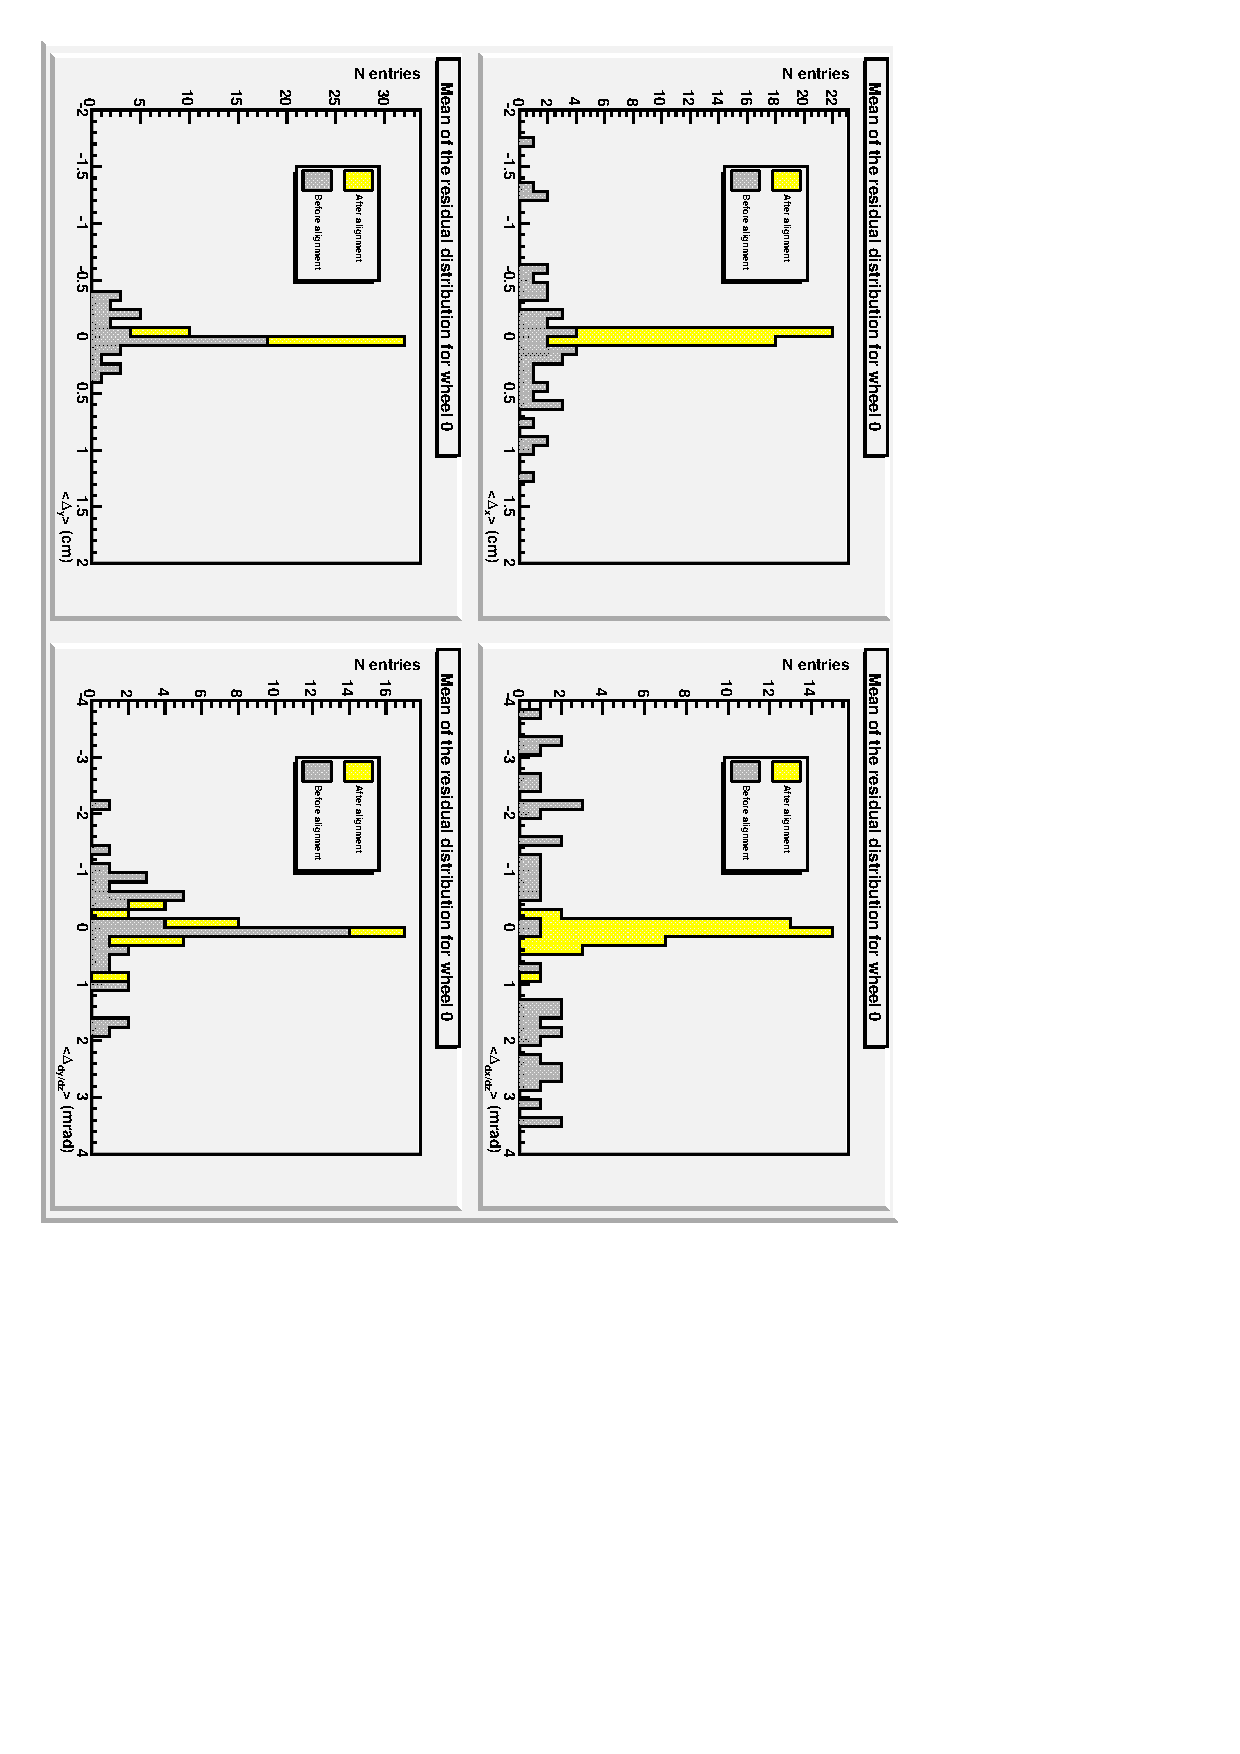
\includegraphics[width=0.7\textwidth, angle=90]{plots/validation/rmdwheel0.pdf}
  }
  \label{fig:valid_RMDYB0}
  \caption{RMD. }
\end{figure}
 

